


% ----------------------------


% \begin{frame}{Lower bounds on  \( M_d(n) \)}
%   \begin{itemize}
%     \item \( M_1(n) = (n-1)^2 + 1 \) (E.SZ).
%     \item  \( M_d(n) \geq n^{(1-1/d)\,n^{d-1}} \)
%   \end{itemize}
%   \pause
%   \begin{proof}{Probabilistic proof}
%       Take \(d=2\), then the bound becomes \(M_2(n)\geq n^{n/2}\).\\
%       Expected number of monotone subarrays of size \(n\) is:
%       \[E=\binom{N}{n}\binom{N}{n}\left(\frac{1}{n!}\right)^n \ll 1\]
%   \end{proof}
% \end{frame}


% ----------------------------


\begin{frame}{}
    \( M_d(n) \): minimum \( N \) such that every \( d \)-dim
  \( N^d \) array has a monotone \( n^d \) subarray.
  \begin{itemize}
    \item $M_1(n) = (n-1)^2 + 1$ \quad (Erd\H{o}s--Szekeres)
    \item $M_d(n) \geq n^{(1-1/d)\,n^{d-1}}$
  \end{itemize}
  \pause
  \begin{proof}{Probabilistic proof sketch ($d=2$)}
      The bound becomes $M_2(n) \geq n^{n/2}$. \\
      Take a uniformly random $N \times N$ array. \\
      By linearity of expectations the expected number of monotone 
      $n \times n$ subarrays is at most
      \[
          E \leq \binom{N}{n}^2 \cdot \frac{4}{(n!)^n} 
          \leq \frac{4N^{2n}}{(n!)^n}\ll1.
      \]
      \pause
      Thus there exists an array with no monotone $n\times n$ subarray.
      Thus $M_2(n) \geq n^{n/2}$.
  \end{proof}
\end{frame}

% ----------------------------

\begin{frame}{Upper bounds}
    \begin{fact}{Previous bounds}
    \begin{itemize}
        \item \(M_2(n)\leq \text{towr}_5(n)\)
        \item \(M_d(n)\leq \text{Ackerman}(n)\)
    \end{itemize}
    \pause
    \end{fact}
    \begin{fact}{Authors}
        \item[\textbf{(i)}] \( \displaystyle M_2(n) \leq 2^{2^{(2+o(1))n}} \)
      \item[\textbf{(ii)}] \( \displaystyle M_3(n) \leq 2^{2^{(2+o(1))n^2}} \)
      \item[\textbf{(iii)}] \( \displaystyle M_d(n) \leq 2^{2^{2^{O_d(n^{d-1})}}}
            \quad \text{for } d \geq 4 \)
    \end{fact}
\end{frame}

% ----------------------------

\begin{frame}{Proof of the bound for \(M_2(n) \le 2^{2^{2n}}\)}
\begin{columns}
\begin{column}{0.65\linewidth}

Take \(N = 2^{2^{2n}}\) and an array of size \(4n^2 \times N\).

By Erdős--Szekeres, each column contains a monotone subsequence of length \(2n\).\\
\onslide<2->{
There are at most \(\binom{4n^2}{2n}\) possible choices of positions, so by pigeonhole,
there exists a set \(R\) of \(2n\) rows and a set \(C\) of columns with
\[
|C| \ge \frac{N}{\binom{4n^2}{2n}} \approx N^{1-o(1)}
\]
such that all columns in \(C\) are monotone on \(R\).\\
}
\onslide<3->{
At least half of these are increasing (or decreasing), so we may assume all columns
in \(C\) are increasing.
}
\end{column}

\begin{column}{0.4\linewidth}
\begin{figure}
\centering
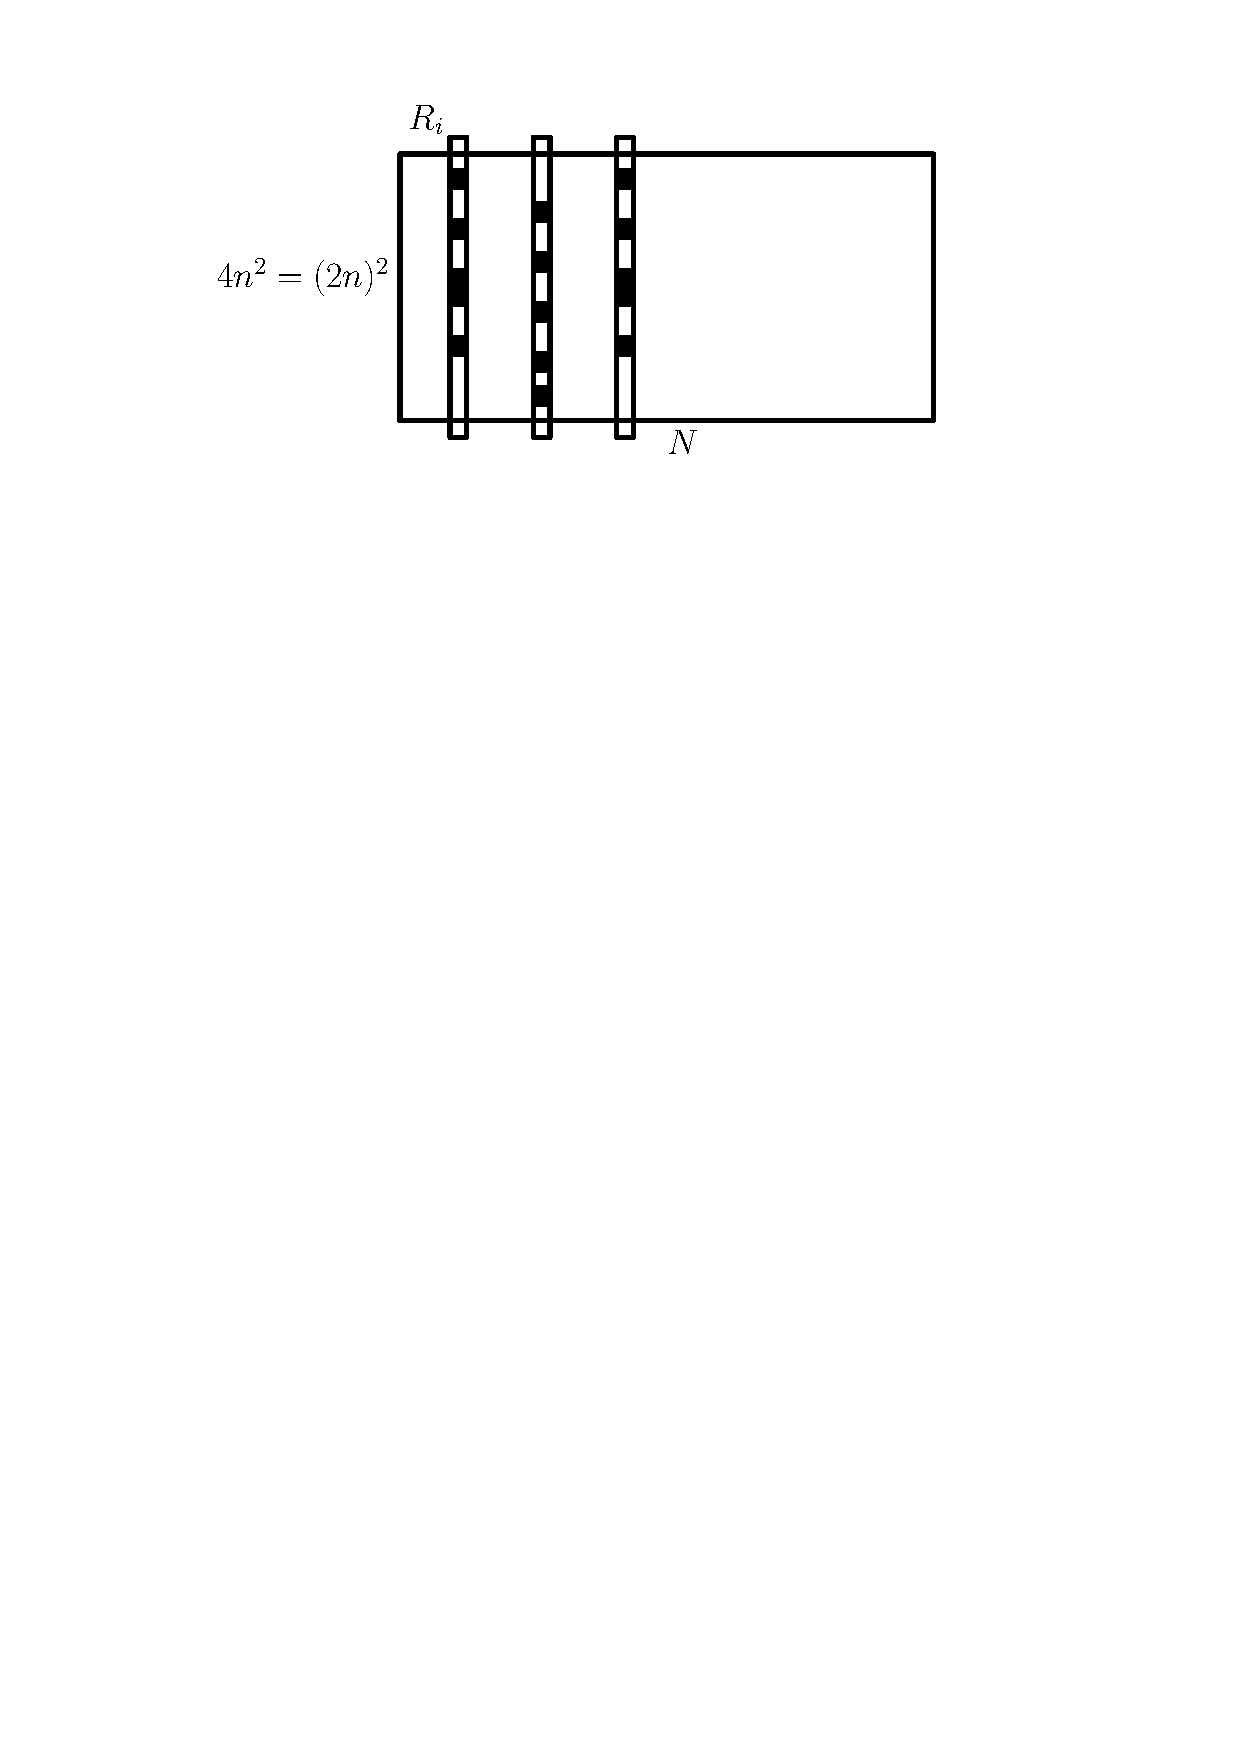
\includegraphics[width=\linewidth]{images/m2_1.pdf}
\end{figure}
\end{column}
\end{columns}
\end{frame}
% ----------------------------


\begin{frame}{Proof of the bound for \(M_2(n) \le 2^{2^{2n}}\)}
\begin{columns}
\begin{column}{0.65\linewidth}
Now iterate Erdős--Szekeres on rows:

At step \(i\), restrict to columns \(C_i\) such that the first \(i\) rows are monotone.
Then
\[
|C_i| \ge |C|^{1/2^i}.
\]
\onslide<2->{
After \(2n\) steps,
\[
|C_{2n}| \ge |C|^{1/2^{2n}} \approx N^{1/2^{2n}}\ge 2n.
\]
}
\onslide<3->{
Thus we obtain a \(2n \times 2n\) subarray where all rows and columns are monotone.
Taking a majority direction among rows gives an \(n \times n\) monotone subarray.
}
\end{column}

\begin{column}{0.4\linewidth}
\begin{figure}
\centering
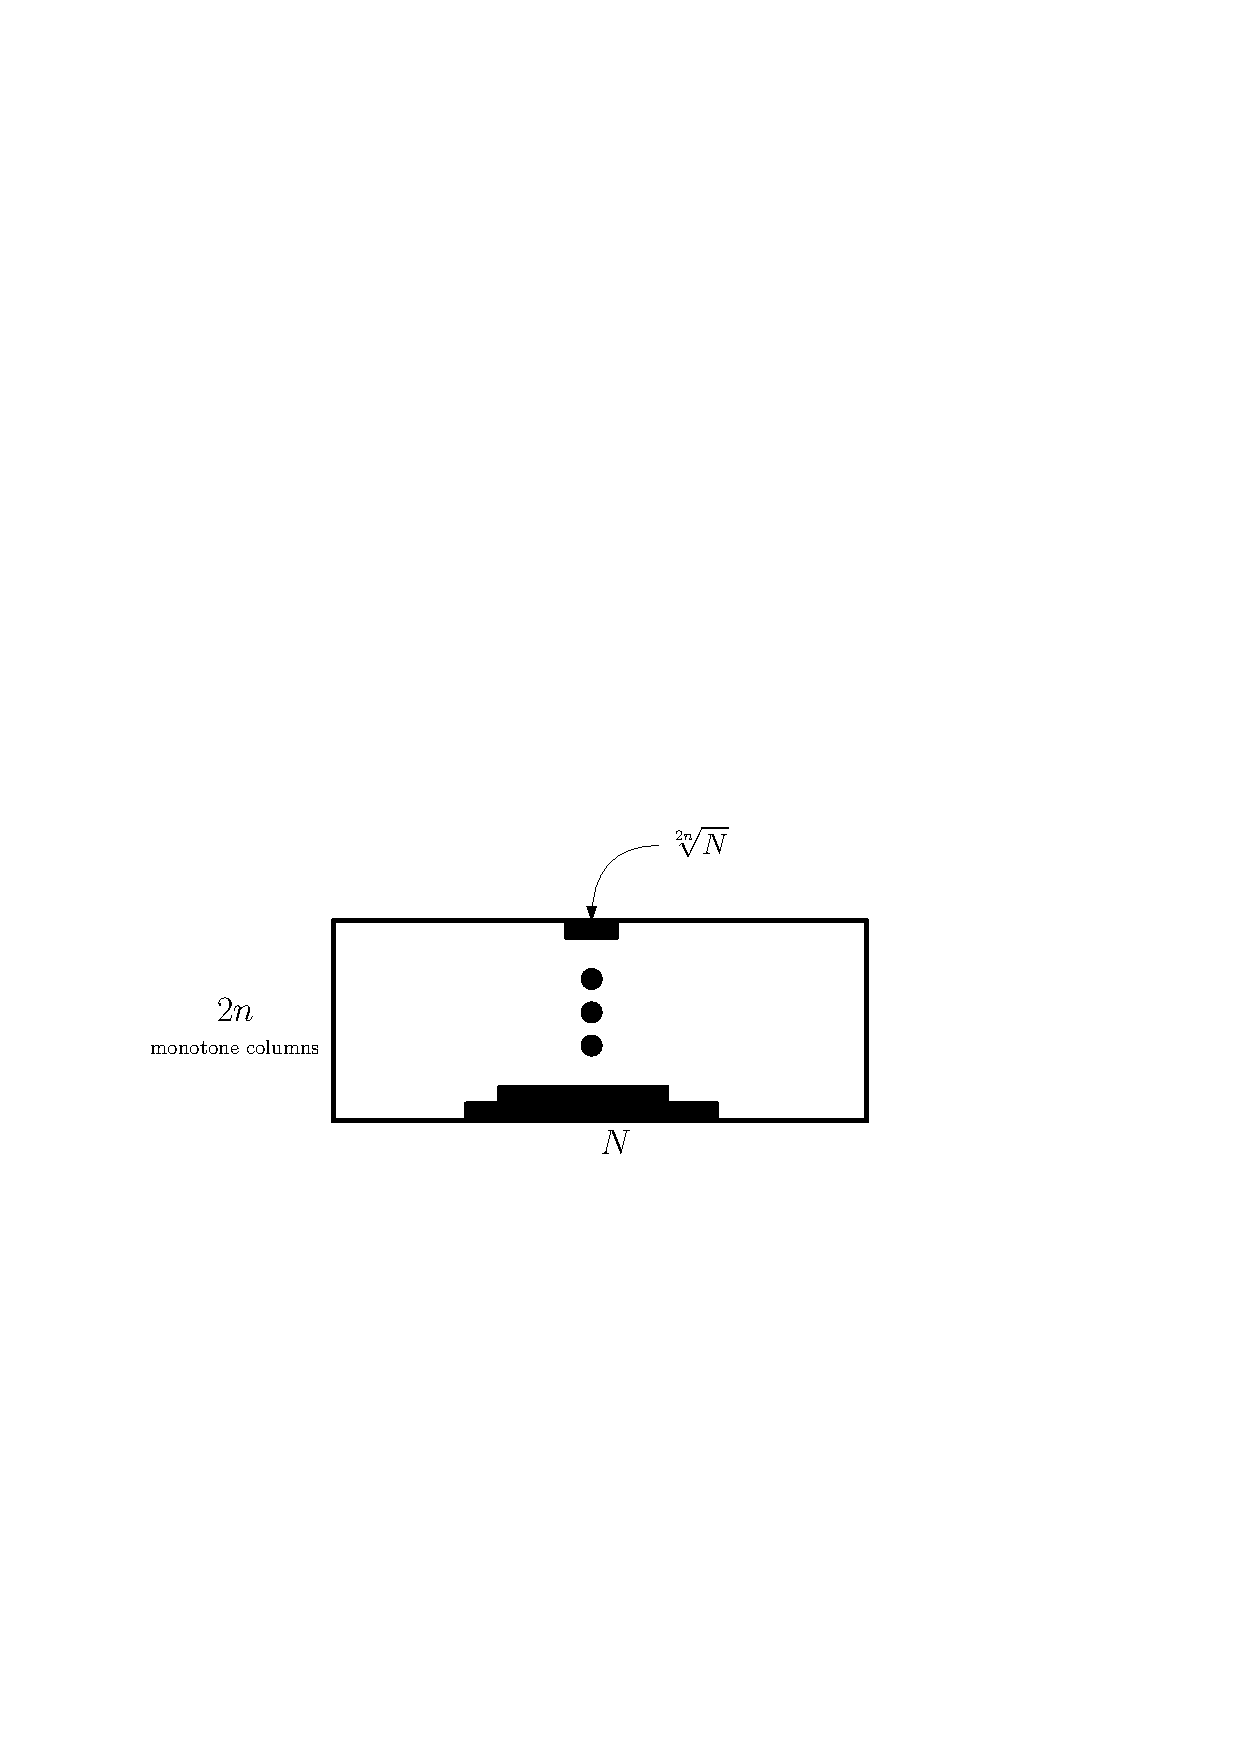
\includegraphics[width=\linewidth]{images/m2_2.pdf}
\end{figure}
\end{column}

\end{columns}
\end{frame}


% ----------------------------


\begin{frame}{Inconsistently Monotone Arrays}
  \begin{ffact}{Inconsistently Monotone Arrays}
    A \( d \)-dimensional array is \textbf{inconsistently monotone} if every
    one-dimensional slice is monotone (but slices along the same direction
    may go in different directions).
  \end{ffact}

  \medskip
    \( M_d'(n) \): minimum \( N \) such that every \( d \)-dim
  \( N^d \) array has an inconsistently monotone \( n^d \) subarray.
    \medskip
    \[M_2(n)\leq M_2'(2n)\]
    \[M_d'(n)\leq 2^{2^{n^{d-1}}}\]
\end{frame}


% ----------------------------

\begin{frame}{Proof of \(M_d'(n)\leq 2^{2^{n^{d-1}}}\)}
    \[
  M_d'(n) \;\leq\; \binom{M_{d-1}'(n)}{n}^{\!d-1} \cdot n^{2n^{d-1}}
\]
Set \( N = \binom{M_{d-1}'(n)}{n}^{d-1} n^{2n^{d-1}} \) and consider an array \( A : [m]^{d-1} \times [N] =S\times N\). We aim to show an inconsistently monotone array of size \(n\).\\
    \pause
  \begin{ffact}{Step 1 — Pigeonhole over heights}\\
  There are \(\binom{m}{n}^{d-1}\) ways to choose the set \(S\).\\
  Thus by pigeonhole principle, there exists a fixed \( S \) and \( H \subseteq [N] \) with
  \[
    |H| \;\geq\; \frac{N}{\binom{m}{n}^{d-1}} \;=\; n^{2n^{d-1}}.
  \]
  such that \(S\times h\) is inconsistently monotone for all \(h \subseteq H\).
  
  \end{ffact}
\end{frame}
\begin{frame}{}
    \[
  M_d'(n) \;\leq\; \binom{M_{d-1}'(n)}{n}^{\!d-1} \cdot n^{2n^{d-1}}
\]
Set \( N = \binom{M_{d-1}'(n)}{n}^{d-1} n^{2n^{d-1}} \) and consider an array \( A : [m]^{d-1} \times [N] =S\times N\). We aim to show an inconsistently monotone array of size \(n\).\\
  \begin{ffact}{Step 2 — Erd\H{o}s--Szekeres along \( H \).}\\
  Label elements of \( S \) as \( s_1,\ldots,s_{n^{d-1}} \).
  Build a nested chain
  \( H_0 \supseteq H_1 \supseteq \cdots \supseteq H_{n^{d-1}} \)
  with \( |H_i| \geq \sqrt{|H_{i-1}|} \), so that \( \{s_j\}\times H_i \)
  is monotone for \( j = 1,\ldots,i \). After \( n^{d-1} \) steps:
  \vspace{-0.5cm}
  \[
    |H_{n^{d-1}}| \;\geq\; |H|^{1/2^{n^{d-1}}} \;\geq\; n.
  \]
  \vspace{-0.5cm}
  Then \(S \times H_{n^{d-1}} \) is inconsistently monotone.
  \end{ffact}
\end{frame}
\begin{frame}{Proof of \(M_d'(n)\leq 2^{2^{n-1}}\)}
    we proved     \[
  M_d'(n) \;\leq\; \binom{M_{d-1}'(n)}{n}^{\!d-1} \cdot n^{2n^{d-1}}
\]
Then by induction using \(\binom{m}{n}\leq m^n\):
\[M_1'(n)=(n-1)^2+1\]
    \[
      M_d'(n)
      \leq \left(2^{2^{n^{d-2}}}\right)^{(d-1)n}\cdot n^{2n^{d-1}}
      = 2^{(d-1)n\cdot 2^{n^{d-2}}+2n^{d-1}\log_2 n}
      = 2^{2^{n^{d-1}}},
    \]
\end{frame}
% ----------------------------


\begin{frame}{}
    \begin{lemma}{Ramsey theory lemma}
    Given k-colouring of vertices of d-dimensional \(N^d\) array there is an \(n^d\) monochromatic subarray if \(2^{Cn^{d-1}}\), where \(C\) is sufficiently large.
    \end{lemma}
    \pause
    \begin{proof}{Proof sketch d=2}
        \begin{itemize}
            \item Each column is a sequence of $N$ cells coloured with $k$ colours
            \item At step $i$, restrict to columns $C_i$ where the first $i$ rows 
            share the same colour. By pigeonhole $|C_i| \geq |C_{i-1}|/k$
            \pause
            \item After $n$ steps: $|C_n| \geq N/k^n$
            \item Apply pigeonhole again on rows: among $N$ rows, 
            some colour class has $\geq N/k$ rows -- pick $n$ of them
            \item Setting $N \geq n \cdot k^{n+1}$ guarantees an $n \times n$ 
            monochromatic subarray
            \pause
            \item For general $d$: iterate over all $d$ dimensions, 
            losing $k^{n^{d-1}}$ at each step, giving $N \geq 2^{Cn^{d-1}}$
        \end{itemize}
    \end{proof}
\end{frame}


%--------------------


\begin{frame}{}
    \begin{theorem}{From inconsistently to consistently}
        Every inconsistently monotone array \(N^d\) has a motone subarray \(n^d\) if \(N=2^{O(n^{d-1})}\)
    \end{theorem}
    \pause
    \begin{proof}{Proof}
    Take an inconsistently monotone array \(A\).\\
    Colour each point \( a \in A \) with its
      \emph{monotonicity pattern}
      \[
        \mathrm{color}(a) = (s_1,\ldots,s_d) \in \{-1,+1\}^d,
        \quad s_i = \begin{cases} +1 & \text{if direction } i \text{ is increasing at } a \\ -1 & \text{otherwise} \end{cases}.
      \]
      By the Ramsey lemma there exists a monochromatic subarray, it is also a monotone subarray.
    \end{proof}
\end{frame}

%--------------------

\begin{frame}{Getting the bound for \(M_d\)}
    \begin{theorem}{Bound on \(M_d'\)}
        \[M_d'(n)\leq 2^{2^{n-1}}\]
    \end{theorem}
    \begin{theorem}{From inconsistently to consistently}
        Every inconsistently monotone array \(N^d\) has a motone subarray \(n^d\) if \(N=2^{O(n^{d-1})}\)
    \end{theorem}
    \pause
    We can combine those proofs to get that:
    \begin{theorem}{Bound on \(M_d\)}
        \[M_d(n)\leq 2^{2^{2^{O(n^{d-1})}}}\]
    \end{theorem}
\end{frame}